\documentclass{book}
\usepackage{graphicx}
\usepackage{float}
\graphicspath{{../img/}}
\author{Matilde Mazzini | Marsha Gomez Gomez}
\begin{document}
    \begin{titlepage}
        \centering
        
\includegraphics[width=6cm]{unipi}
        \vfill
        \vspace{1.5cm}
        {\huge\textsc{Advance Data Mining and Machine Learning}\par}
        {\Large
            Games Genre Prediction\\
            First Semester 2019\\
            \vskip2cm
            Matilde Mazzini | Marsha Gomez\\
            \vskip2cm
            \today
        }    
        \vfill
        \vfill
    \end{titlepage}
    \tableofcontents

    \section*{Abstract}
    \paragraph{}
    Websites like PlayStation Now, Steam and Origin, offer lists of games based on genres, this makes it easier for a user to select the game that interests you based on the genre is motivated towards. Tagging of games is a complex process and usually involves a labor-intensive process where the games are assigned to one or more Genres based on the proposals sent by the users and consumers. If we can systematize this process of game tagging, not only will it be fast, save human effort but it will be more accurate than an untrained human as well.

    \chapter{Introduction}
    \paragraph{}
    Public games database such RAWG provides genre information to assist searching. The tagging of games genres is still a manual process which involves the collection of users suggestions and consumers. Games are often registered with inaccurate genres. Automatic genres classification of a game based on its synopsis not only speeds up the classification process by providing a list of suggestion but the result may potentially be more accurate than an untrained human. We will collect data using one of many available apis on internet and compile a data set wich will be primarily based on \textit{GDB (Game Data Base)}. We will rely on text analysis of the Plot/Summary of the movie data collected and train our classifier using text analysis techniques

    \chapter{Data Collection}
    \paragraph{}

    The Data Set on this project is a set of text files from GDB.They contain 80,000 games and 65,000 of genre information of games. For this project \textbf{65,000} \textit{unique} titles at wich both the description and genre information were available were chosen and randomly split into 80\% and 20\% sets. The former was used for training while the latter for testing.

    Note that a game can be (and often so) associated with \textbf{more than one} genres. There are 12 listed genres in the GDB data set and only the \textbf{7} (denoted as \textit{L}) most commong genres were used in this project. The genres names and percentages of games in them are: \textit{action (22\%), adventure (15\%), puzzle (14\%), RPG (10\%), simulation (9\%), strategy (9\%), Shooter (7\%), sports (4\%), racing (3\%) educational (2\%), fighting (2\%), BoardGames (3\%)}
    \begin{table}[H]\label{tab:genre}
        \centering
        \begin{tabular}{|p{3cm}|p{3cm}|p{3cm}|}
            \hline
            \multicolumn{3}{|c|}{Genres List} \\
            \hline
                    Genre & Count & Porcentage \\
            \hline
                    Action & 6848 & 22 \% \\
                Adventure & 4725 & 15 \% \\
                    Puzzle & 4412 & 14 \% \\
                        RPG & 3105 & 10 \% \\
                Simulation & 2745 & 9 \% \\
                Strategy & 2660 & 9 \% \\
                    Shooter & 2101 & 7 \% \\
                    Sports & 1122 & 4 \% \\
                    Racing & 1000 & 3 \% \\
                Educational & 549 & 2 \% \\
                Fighting & 593 & 2 \% \\
                BoardGames & 640 & 3 \% \\
            \hline 
        \end{tabular}
        \caption{Genres Detail.}
    \end{table}

    \begin{figure}[H]\label{fig:plotGenre}
        \centering
        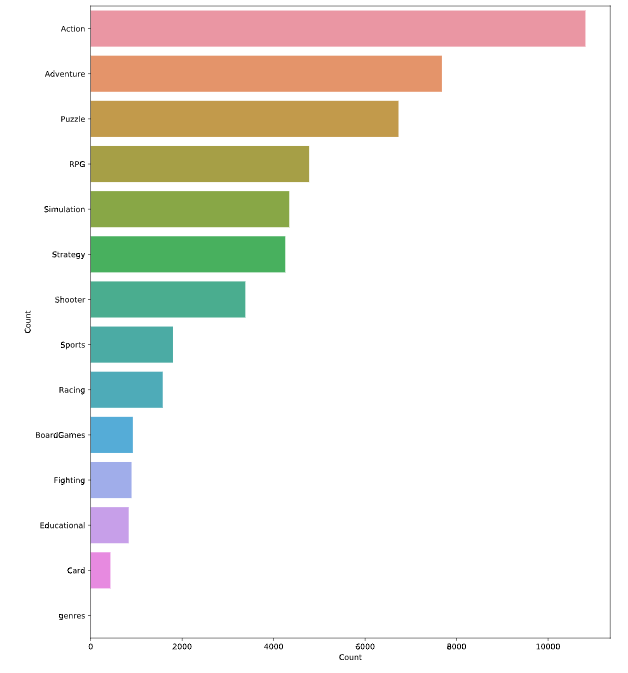
\includegraphics{plot-genres}
        \caption{Graph genres representation.}
    \end{figure}

    \chapter{Data Preprocesing}
    \chapter{Data Mining}
    \chapter{Conclusions}

    \listoftables
    \listoffigures

\end{document}
